\section{Allele-level audit: AlphaMissense saturates on panel alleles (MyVariant.info)}
The earlier audits worked at gene level. A mutation-based detection panel calls
\emph{alleles}, so we asked three allele-level questions. We fetched every
somatic mutation in the four panel genes and in eight long, frequently mutated
passenger genes (TTN, MUC16, RYR1, LRP1B, CSMD3, USH2A, SYNE1, FLG) from seven
hg19 PDAC cohorts on cBioPortal (3,134 patients carrying at least one mutation in these genes; legacy \texttt{paad\_tcga} and
the two smaller MSK cohorts were excluded to avoid double-counting patients),
7,395 mutation records in total. Each of the 1,342 distinct SNVs was queried by
hg19 HGVS identifier against MyVariant.info (batch POST), which returned CADD
phred, dbNSFP AlphaMissense and REVEL scores, and ClinVar RCV significance
(99.9\% of SNV records resolved; \texttt{results/myvariant\_variants.csv}).
Trinucleotide context for every missense allele came from the UCSC Genome
Browser REST API (hg19); the reference base matched the cBioPortal allele for
all 1,019 of 1,019 alleles (\texttt{results/myvariant\_allele\_context.csv}).

\paragraph{Positive control (passes).} Panel missense alleles score far above
passenger missense on every predictor (Table~\ref{tab:myvariant}; AlphaMissense
AUROC 0.936, $p=6.3\times10^{-126}$). This calibrates the annotations; had it failed, the
rest would be void.

\paragraph{Within-panel recurrence: AlphaMissense has no room left.} We then
asked whether a predictor ranks the panel's alleles by how many patients carry
them (recurrent $\ge3$ patients vs.\ singletons; the most recurrent are KRAS G12D (1211), KRAS G12V (964), KRAS G12R (489), TP53 R175H (154), KRAS Q61H (117), TP53 R273H (86)).
AlphaMissense does not: pooled AUROC 0.537 ($p=0.19$), and it fails in both
cohort splits. The reason is a ceiling: 86.2\% of panel \emph{singleton}
missense alleles already exceed the published likely-pathogenic threshold
(0.564), and 72.9\% exceed 0.9. REVEL and CADD do track recurrence in the
pooled data (AUROC 0.625 and 0.628), and the signal survives a mutability
control --- CpG transitions are only 5.9\% of panel alleles but are
enriched among recurrent ones ($\rho=0.12$, $p=0.0038$), and restricting to
non-CpG alleles leaves REVEL $\rho=0.18$ and CADD $\rho=0.18$. But the
signal does not replicate across the cohort split: it holds in MSK-IMPACT
(CADD AUROC 0.648) and is null in the pooled WES/WGS cohorts (CADD AUROC
0.543, $p=0.27$, recurrent $=\ge2$ patients). REVEL is also trained on
disease-mutation databases that contain the TP53 hotspots, so its advantage is
partly circular. \textbf{Verdict:} no predictor gives a cohort-robust ranking of
panel alleles; the robust finding is the negative one, that AlphaMissense
cannot rank them at all. We name this the \emph{AlphaMissense panel ceiling} and state it falsifiably: in any new PDAC cohort with $\ge100$ recurrent panel missense alleles, AlphaMissense AUROC for recurrent vs singleton will stay below 0.60; an AUROC $\ge0.60$ with $p<0.01$ refutes it.

\begin{table}[h]\centering\footnotesize
\caption{Allele-level predictor audit. Columns: median score (panel / passenger
missense alleles); AUROC panel vs passenger; AUROC recurrent vs singleton
within panel (pooled, MSK-IMPACT, WES/WGS); Spearman $\rho$ recurrence vs score
on non-CpG panel alleles.}\label{tab:myvariant}
\begin{tabular}{p{2.0cm}p{0.9cm}p{0.9cm}p{1.0cm}p{1.0cm}p{2.0cm}p{2.0cm}p{2.0cm}}
\hline
Predictor & panel & pass. & drv/pass & pooled & MSK & WES/WGS & non-CpG $\rho$ \\ \hline
AlphaMissense & 0.993 & 0.188 & 0.936 & 0.537 & 0.549 ($p=0.12$) & 0.517 ($p=0.65$) & 0.055 ($p=0.21$) \\
REVEL & 0.902 & 0.222 & 0.947 & 0.625 & 0.613 ($p=0.00039$) & 0.531 ($p=0.43$) & 0.177 ($p=6.6\times10^{-5}$) \\
CADD phred & 27.500 & 21.200 & 0.848 & 0.628 & 0.648 ($p=2.8\times10^{-6}$) & 0.543 ($p=0.27$) & 0.181 ($p=3.7\times10^{-5}$) \\
\hline\end{tabular}\end{table}

\paragraph{CDKN2A is the exception.} Patient-weighted, KRAS 99.9\%, TP53 98.2\% and
SMAD4 98.3\% of missense carriers hold an AlphaMissense likely-pathogenic allele,
but only 55.4\% of CDKN2A missense carriers do. One candidate explanation (not tested here) is that
the scores are defined on a single canonical protein, while CDKN2A also
encodes p14$^{ARF}$ from an alternate reading frame, so an allele's effect on
that product is not scored. We treat the low scores as a limit of the
predictor, not as evidence that those alleles are passengers.

\paragraph{How many panel calls rest on unsupported alleles?} Calling an
alteration \emph{supported} if it is truncating, ClinVar pathogenic/likely
pathogenic, or AlphaMissense likely-pathogenic, 99.4\% of the 3,115
panel-positive patients carry at least one supported alteration (ClinVar P/LP
alone: 97.8\%); 19 patients carry only unsupported alterations (mostly
in-frame indels and low-scoring missense). The denominator is panel-positive
patients only, so this is a bound on annotation support, not on sensitivity.

\begin{figure}[h]\centering
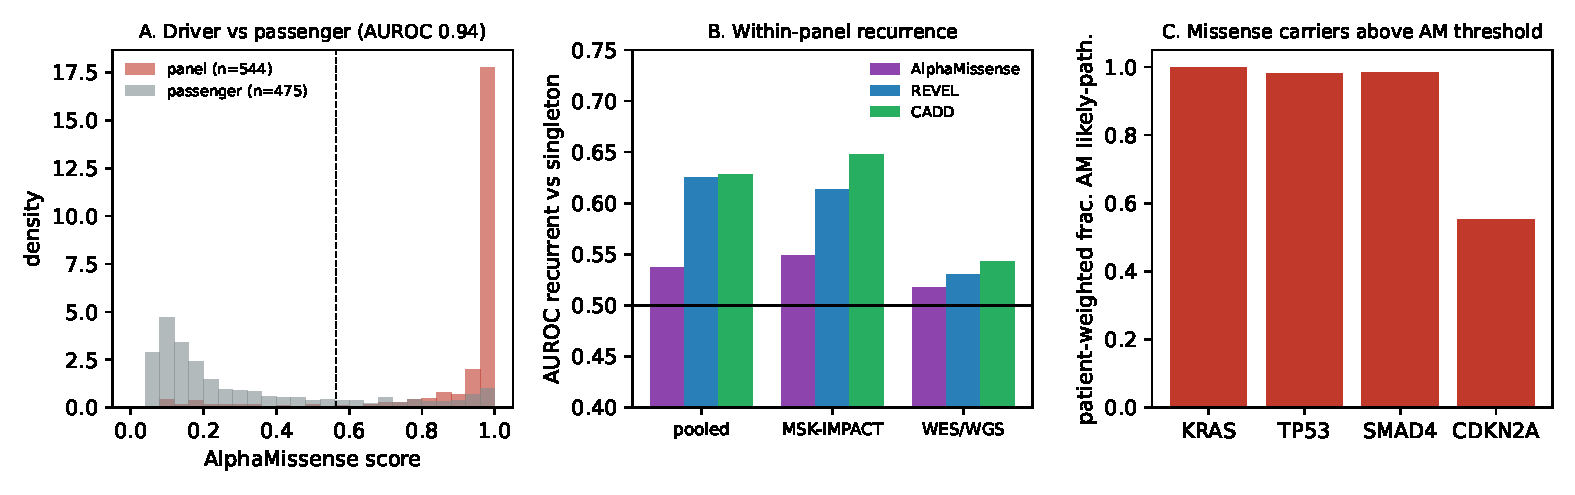
\includegraphics[width=\linewidth]{figs/fig_myvariant.pdf}
\caption{MyVariant allele audit. A: AlphaMissense separates driver from
passenger missense. B: no predictor ranks panel alleles by recurrence
robustly across cohorts. C: CDKN2A missense carriers fall below the
AlphaMissense threshold far more often than the other panel genes.}
\label{fig:myvariant}\end{figure}
